\chapter{Suggestions to Improve The Existing System} \label{suggestions}

\section{System Perspective}
\begin{figure}[H]
    \centering
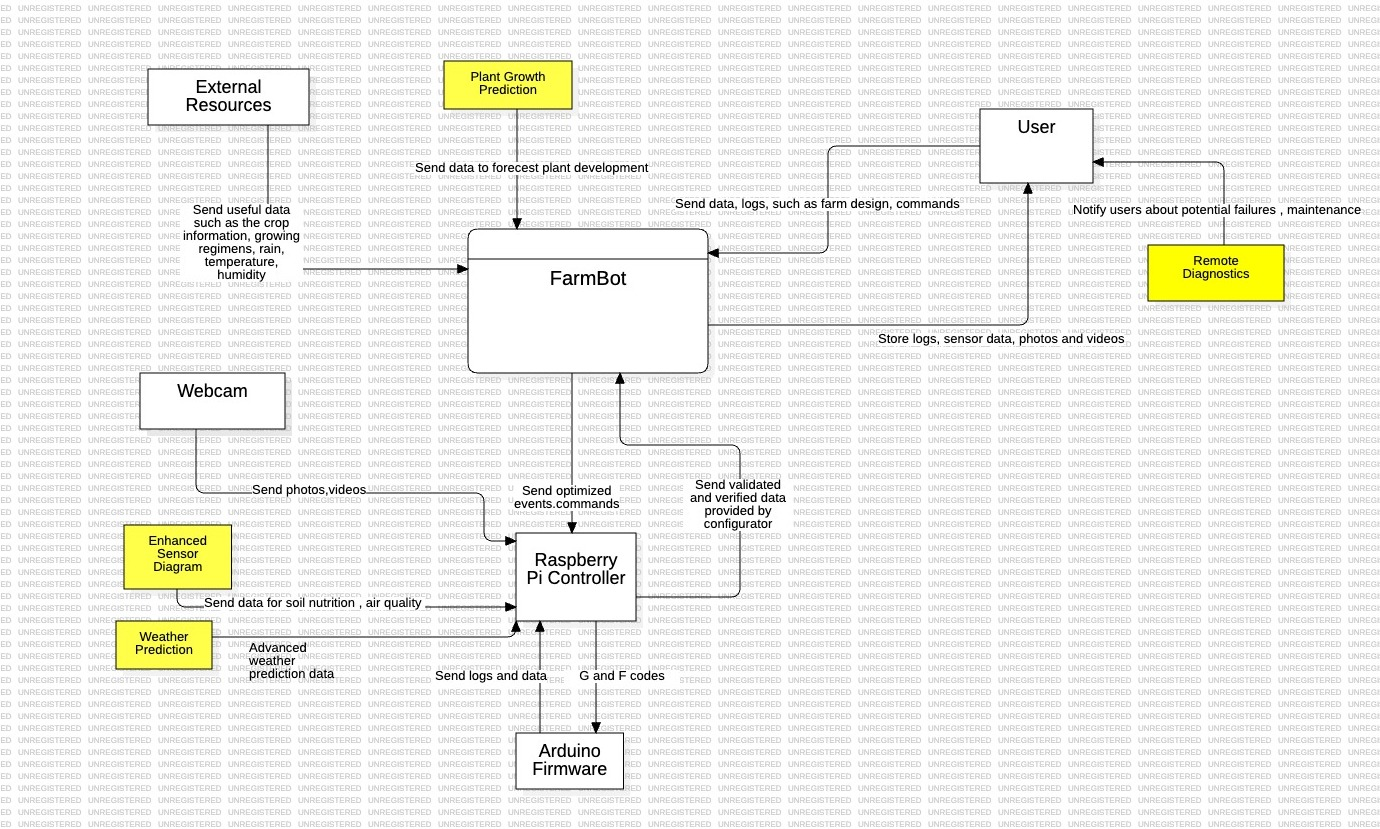
\includegraphics[scale=0.37]{./Figures/farmbot_context_diagram_suggested.jpg}
\caption{FarmBot Context Diagram with Suggestions}
\end{figure}


The system's architecture, designed to automate precision farming through FarmBot, interacts with various external and internal components. This section discusses improvements in the context of the system's interaction with its environment, highlighting four key areas for enhancement.

\subsection{Enhanced Sensor Integration}
\textbf{Context and Explanation:} Integrating a broader range of environmental sensors into FarmBot's system can significantly improve its adaptive capabilities. Enhanced sensors for detecting soil nutrition and air quality will allow FarmBot to respond more dynamically to the needs of the plants and the conditions of their environment. This could involve incorporating new sensor types that measure specific nutrient levels in the soil or detect pollutants in the air that could affect plant growth.

\textbf{Suggested Improvements:}
\begin{itemize}
    \item Incorporate nitrogen, phosphorus, and potassium (NPK) soil sensors to optimize fertilizer application.
    \item Add air quality sensors to monitor the presence of pollutants that could harm plant health.
    \item Develop a sensor data aggregation module in the software to analyze data from multiple sources for comprehensive environmental assessment.
\end{itemize}

\subsection{Advanced Weather Prediction Integration}
\textbf{Context and Explanation:} Weather plays a crucial role in farming operations. By integrating advanced weather prediction models that utilize machine learning to process historical weather data, FarmBot can proactively adjust its operations—such as watering, planting, and harvesting schedules—based on accurate weather forecasts.

\textbf{Suggested Improvements:}
\begin{itemize}
    \item Partner with advanced weather prediction services or invest in the development of proprietary weather prediction algorithms.
    \item Implement machine learning models that can analyze patterns in long-term weather data to forecast local weather conditions with higher accuracy.
    \item Automatically adjust FarmBot's operational schedules based on weather predictions to optimize plant growth and resource usage.
\end{itemize}

\subsection{Plant Growth Prediction Models}
\textbf{Context and Explanation:} Predicting plant growth stages and harvest times can significantly enhance the scheduling efficiency of FarmBot. Integrating plant growth prediction models that leverage historical growth data and current environmental conditions will allow for more precise planning of farming operations.

\textbf{Suggested Improvements:}
\begin{itemize}
    \item Develop or integrate existing plant growth models into FarmBot's software, tailored to the variety of plants supported by the system.
    \item Use accumulated data from FarmBot's operations and external data sources to refine and validate the growth models continuously.
    \item Provide users with predictions on growth stages and optimal harvest times, enhancing the planning and execution of farming tasks.
\end{itemize}

\subsection{Remote Diagnostics and Proactive Maintenance}
\textbf{Context and Explanation:} Ensuring the reliability of FarmBot's operations requires a system for early detection of potential failures or maintenance needs. Implementing a framework for remote diagnostics and proactive maintenance can help in identifying issues before they lead to system downtime.

\textbf{Suggested Improvements:}
\begin{itemize}
    \item Develop diagnostic algorithms that monitor system performance and predict potential failures based on operational data and sensor readings.
    \item Implement a maintenance scheduling module that alerts users to upcoming maintenance tasks and suggests optimal times for their completion.
    \item Allow for remote firmware updates and system checks to ensure that FarmBot operates with the latest software and within optimal performance parameters.
\end{itemize}

Each of these improvements aims to enhance the adaptability, efficiency, and reliability of the FarmBot system, leveraging advanced technologies and data-driven strategies to optimize precision farming operations.


\section{External Interfaces}

\begin{figure}[H]
    \centering
\includesvg[inkscapelatex=false, scale=0.42]{./Figures/external_interface_class_diagram_suggestions.svg}
\caption{Class Diagram for External Interfaces}
\end{figure}


This section outlines the external interfaces of the FarmBot system, highlighting the integration of both original and suggested interfaces to enhance system functionality. The context diagram (not included here) visually represents these interfaces and their connections. The following descriptions detail how suggested interfaces can complement and expand the capabilities of the existing system.

\subsection{Suggested External Interfaces}

\textbf{Plant Database API}
\begin{itemize}
    \item \textbf{Purpose:} To enrich FarmBot's knowledge base with extensive plant species data and their specific growth requirements, facilitating more informed decision-making for planting strategies.
    \item \textbf{Improvements:} Integration of a comprehensive plant database allows for automated, species-specific care routines, optimizing growth conditions for a diverse range of crops and enhancing yield efficiency.
\end{itemize}

\textbf{GPS Communication Interface}
\begin{itemize}
    \item \textbf{Purpose:} To provide precise geolocation capabilities for FarmBot, enabling accurate mapping of the farming area and plant locations.
    \item \textbf{Improvements:} With accurate GPS data, FarmBot can perform tasks with enhanced precision, such as targeted watering or planting, reducing resource waste and improving operational efficiency.
\end{itemize}

\textbf{Weather API}
\begin{itemize}
    \item \textbf{Purpose:} To fetch real-time and forecasted weather data, allowing FarmBot to adapt its operations based on current and upcoming weather conditions.
    \item \textbf{Improvements:} Weather adaptability ensures that FarmBot can make proactive adjustments to its routines, such as delaying watering before rain, thus optimizing resource use and protecting plants from adverse weather.
\end{itemize}

\textbf{Diagnostic and Logging API}
\begin{itemize}
    \item \textbf{Purpose:} To collect detailed diagnostics and operational logs from FarmBot, facilitating remote troubleshooting and system optimization.
    \item \textbf{Improvements:} Enhanced diagnostic capabilities enable predictive maintenance and quick resolution of issues, improving system reliability and uptime.
\end{itemize}

\subsection{Integration with Existing Interfaces}

The suggested interfaces complement the existing system's capabilities, forming a cohesive and intelligent farming solution:
\begin{itemize}
 

   \item  The \textbf{User Interface API} becomes a more powerful tool for users, offering access to a broader range of data and controls, from selecting plants from the \textbf{Plant Database API} to viewing weather forecasts via the \textbf{Weather API}.
   \item The \textbf{Sensor Data Interface} and \textbf{GPS Communication Interface} work in tandem to provide environmental and locational data, enhancing the precision of FarmBot's operations.
   \item  Integration of the \textbf{Diagnostic and Logging API} with the \textbf{Remote Update API} ensures that FarmBot's software remains up-to-date and operates efficiently, with maintenance and updates informed by comprehensive diagnostic data.
\end{itemize}
\subsection{Improvement Recommendations}

To fully leverage the potential of the suggested external interfaces, the following recommendations are proposed:

\begin{itemize}
  

  \item  Data Synchronization: Implement robust data synchronization mechanisms between the FarmBot system and the external APIs to ensure real-time accuracy and responsiveness.
  \item  User-Centric Design: Continuously refine the User Interface API to present the enriched data and controls in an intuitive and accessible manner, enhancing the user experience.
  \item  Security and Privacy: Ensure all external communications are encrypted, and data privacy is maintained, especially when integrating third-party APIs like weather services and GPS data providers.

By incorporating these suggested external interfaces and adhering to the improvement recommendations, the FarmBot system can achieve significant advancements in automation, efficiency, and user engagement.
\end{itemize}
\section{Functions}

\begin{figure}[H]
    \centering
\includesvg[inkscapelatex=false, scale=0.42]{./Figures/UseCaseExtended.svg}
\caption{Use Case Diagram with Suggestions}
\end{figure}

\begin{table}[H]
\centering
\footnotesize
\begin{tabular}{|p{3.5cm}|p{8.5cm}|}
\hline
\textbf{Use case name}    & Internal Community Feed\\
\hline
\textbf{Actors}           & Farmbot App, Users \\
\hline
\textbf{Description}      & Embed the FarmBot Community Blog into the app for easy integration of utilities, schedule sharing, etc. \\
\hline
\textbf{Data}             & User profile info, recent activities, image sharing, garden layout, planting history\\
\hline
\textbf{Preconditions}    & Active internet connection and data sharing permissions. \\
\hline
\textbf{Stimulus}         & FarmBot users connect and interact via. social tab. \\
\hline
\textbf{Basic flow}       & Users share experiences through the social portal $\rightarrow$ Other users interact with content. \\
\hline
\textbf{Alternative flow} & Importation of the data and activities posted on the original community page. \\
\hline
\textbf{Exception flow}   & Connectivity and legal social platform issues. \\
\hline
\textbf{Post conditions}  & Users interact and improve the platform through bug reports and implementation suggestions. \\
\hline
\end{tabular}
\caption{Use Case Model for Internal Community Feed}
\end{table}

\begin{figure}[H]
    \centering
\includesvg[inkscapelatex=false, scale=0.7]{./Figures/CommunityActivityDiagram1.svg}
\caption{Activity Diagram for Internal Community Feed}
\end{figure}

\begin{table}[H]
\centering
\footnotesize
\begin{tabular}{|p{3.5cm}|p{8.5cm}|}
\hline
\textbf{Use case name}    & Analysis-based Planting \\
\hline
\textbf{Actors}           & Scheduler, User, Farmbot \\
\hline
\textbf{Description}      & Use past crop data to improve predictions and plant crops to have higher yields. Use historical data to build on the already existing analysis feature. Add past plant performance as an additional parameter to predict plant growth performance\\
\hline
\textbf{Data}             & Past harvest data, weather data, geospatial data, soil quality and nutrient data, user specifications \\
\hline
\textbf{Preconditions}    & FarmBot has harvested at least one crop cycle in the same location at the same season. \\
\hline
\textbf{Stimulus}         & User decides to optimize scheduling and planting using the past data. \\
\hline
\textbf{Basic flow}       & One crop cycle is completed $\rightarrow$ The data from the previous operation is used to optimize the next one. \\
\hline
\textbf{Alternative flow} & User opts to not use past data and planning is done as standard. \\
\hline
\textbf{Exception flow}   & Past data is non-existent or corrupt. There are new variables introduced making the data obsolete. \\
\hline
\textbf{Post conditions}  & Crop planning is done better resulting in higher yields. \\
\hline
\end{tabular}
\caption{Use Case Model for Analysis-based Planting}
\end{table}

\begin{figure}[H]
    \centering
\includesvg[inkscapelatex=false, scale=0.8]{./Figures/AnalysisStateDiagram.svg}
\caption{State Diagram for Analysis-based Planting}
\end{figure}

\begin{table}[H]
\centering
\footnotesize
\begin{tabular}{|p{3.5cm}|p{8.5cm}|}
\hline
\textbf{Use case name}    & Phenotype Comparison Tracker \\
\hline
\textbf{Actors}           & User, FarmBot \\
\hline
\textbf{Description}      & An automated dashboard for the tracking of scientific experiments on plant genetics and phenotype results. The FarmBot software is extended to support internal experimentation to support the scientific use of the system. Seed labeling and crop tracking is embedded to the system. \\
\hline
\textbf{Data}             & Seed type, planting depth, spacing, garden layout, planting coordinates, genetic differences, test batch, control batch \\
\hline
\textbf{Preconditions}    & All other variables are held constant except seed types of the same plant. \\
\hline
\textbf{Stimulus}         & A hypothesis is tested regarding the effects of plant genes on growth and yield. \\
\hline
\textbf{Basic flow}       & Experiment is conducted on a batch $\rightarrow$ The results are automatically analyzed and stored by the FarmBot system. \\
\hline
\textbf{Alternative flow} & Plants are sown and harvested normally. \\
\hline
\textbf{Exception flow}   & Additional variables are introduced by accident, disabling the experiment. \\
\hline
\textbf{Post conditions}  & Seeds are specifically tracked, making the experiment easier to conduct with less human error. \\
\hline
\end{tabular}
\caption{Use Case Model for Phenotype Comparison Tracking}
\end{table}

\begin{table}[H]
\centering
\footnotesize
\begin{tabular}{|p{3.5cm}|p{8.5cm}|}
\hline
\textbf{Use case name}    & Auto-Farmer \\
\hline
\textbf{Actors}           & FarmBot, User, Scheduler \\
\hline
\textbf{Description}      & Automate the process of planting seeds, watering, weeding, fertilizing, and other activities to make the system fully autonomous. The user is only tasked with base level error handling. \\
\hline
\textbf{Data}             & Crop state, planting options, plant health, schedule, weather data \\
\hline
\textbf{Preconditions}    & FarmBot is operational and loaded with the correct seed types, fertilizer, and water source. \\
\hline
\textbf{Stimulus}         & The user specifies farming choices through the control interface such as plant types, maintenance frequency, and fertilizer amount. Constant weather data is supplied to the system. \\
\hline
\textbf{Basic flow}       & User sets up the system with its parameters $\rightarrow$ FarmBot plants seeds according to the specified parameters and does continuous up-keeping of the plants automatically. \\
\hline
\textbf{Alternative flow} & AutoFarmer is engaged only for certain specific time frames. \\
\hline
\textbf{Exception flow}   & Software or hardware errors are introduced or the system runs out of resources. \\
\hline
\textbf{Post conditions}  & The system constantly tends to the crops allowing it to operate autonomously. \\
\hline
\end{tabular}
\caption{Use Case Model for AutoFarmer}
\end{table}

\begin{figure}[H]
    \centering
\includesvg[inkscapelatex=false, scale=0.65]{./Figures/AutofarmerStateDiagram.svg}
\caption{State Diagram for AutoFarmer}
\end{figure}

\section{Logical Database Requirements}
\begin{figure}[H]
    \centering
\includesvg[inkscapelatex=false, scale=0.42]{./Figures/LogicDiagramExtended.svg}
\caption{Logical Database Class Diagram with Suggestions}
\end{figure}


This section details the enhancements to the FarmBot system's logical database, specifically focusing on the addition of new attributes to Plant Data, Environmental Data, and Scheduling Data. These improvements aim to refine FarmBot's operational efficiency, adaptability, and data analytics capabilities.

\subsection{Enhancements to Plant Data}

\textbf{Plant Data} has been augmented with the following attributes to provide a more comprehensive understanding of each plant's performance and requirements:

\begin{itemize}
    \item \textbf{plantPastPerformanceVariance (Float):} Measures the variance in past performance of plants, aiding in the prediction of future growth patterns and identifying plants that deviate from expected growth trajectories.
    \item \textbf{plantEnvironmentResponse (Float):} Quantifies each plant's responsiveness to environmental conditions, enabling more personalized care strategies that adapt to the plant's specific needs.
    \item \textbf{plantGeneticData (Object):} Contains genetic information of the plants, supporting advanced analysis for breeding optimization and genetic resilience to pests or diseases.
\end{itemize}

\subsection{Enhancements to Environmental Data}

\textbf{Environmental Data} now includes attributes that capture broader ecological and meteorological factors:

\begin{itemize}
    \item \textbf{knownPests (Object):} A record of pests known to affect the farming area, facilitating targeted pest management strategies.
    \item \textbf{weatherAnomalies (String):} Describes historical weather anomalies in the area, providing insights for better preparation against unusual weather patterns.
    \item \textbf{droughtSeason (Boolean):} Indicates whether the current season is prone to drought, aiding in water conservation efforts and drought-resistant planting decisions.
\end{itemize}

\subsection{Enhancements to Scheduling Data}

\textbf{Scheduling Data} has been enhanced with attributes focused on maintenance and operational recording:

\begin{itemize}
    \item \textbf{preventiveMaintenance (Object):} Outlines scheduled maintenance activities for FarmBot's machinery, aiming to prevent equipment failure and extend the system's lifespan.
    \item \textbf{recordingSchedule (Object):} Specifies the schedule for recording various operational data points, ensuring comprehensive data collection for analysis and optimization.
\end{itemize}

\subsection{Class Diagram with Associations}
% In the class diagram, these newly added attributes would be illustrated as part of their respective classes. Associations might include:
% - "Plant Data" linked with "Scheduling Data" to adjust care schedules based on plant genetics and environmental response.
% - "Environmental Data" associated with "Plant Data" to correlate known pests and weather anomalies with plant health and performance.
% - "Scheduling Data" connected to "Diagnostic and Logging API" to ensure maintenance and data recording activities are logged for future reference.

\textbf{Implementation Considerations:}
Incorporating these attributes requires updating the FarmBot software to leverage this enriched data for operational decision-making. This might involve algorithm updates, user interface adjustments for data visualization, and enhanced analytics capabilities to interpret the new data types.

These database enhancements are poised to significantly improve FarmBot's precision agriculture capabilities, making the system more responsive to plant and environmental variables and proactive in maintenance scheduling. The goal is to optimize plant health, yield, and system reliability through data-driven insights.


\section{Design Constraints}

To further enhance the FarmBot system, it is vital to address and adapt to additional design constraints that arise from proposed improvements:

\textbf{Data Privacy and Security:} With the integration of advanced data analytics and genetic information, ensuring the privacy and security of data becomes paramount. Adherence to data protection regulations like GDPR for users' and plants' genetic data is mandatory.

\textbf{Advanced Sensor Compatibility:} The incorporation of enhanced sensors for soil nutrition and air quality demands compatibility with an expanded range of sensor technologies. This necessitates modular and adaptable software drivers and interfaces.

\textbf{Weather Prediction Technologies:} The integration of advanced weather prediction requires handling large datasets and complex algorithms, which may constrain system processing capabilities and require optimization for efficient data processing.

\textbf{Resource Intensity:} The improvements in predictive maintenance, plant growth modeling, and environmental responsiveness increase the system's computational and energy resources. Optimizing for low-power operations and efficient data processing will be essential.

\section{System Quality Attributes}

Improvements to the FarmBot system should prioritize the following quality attributes to ensure the system's effectiveness and user satisfaction:

\textbf{Security:} Enhancements in data analytics and personalization features increase the need for robust security measures to protect user and plant data against unauthorized access and cyber threats.

\textbf{Performance:} Advanced functionalities, such as real-time environmental monitoring and predictive analytics, require the system to process and respond to data efficiently, maintaining high performance without lag.

\textbf{Adaptability:} The system must be flexible to accommodate new sensors, data models, and user preferences without significant overhauls, allowing for seamless updates and integration of new features.

\textbf{User Experience:} With the addition of complex data analytics and more detailed control options, maintaining an intuitive and user-friendly interface is crucial to ensure that users of all technical levels can effectively interact with the system.

\section{Supporting Information}

The suggested improvements to the FarmBot system necessitate updated and comprehensive supporting information:

\textbf{Updated Documentation:} Detailed documentation covering new sensors, weather prediction integration, and plant growth models will be essential for users and developers to understand and leverage the system's enhanced capabilities.

\textbf{Educational Resources:} To aid in the adoption of new features and technologies, providing updated educational resources and tutorials will help users maximize the benefits of the system's improvements.

\textbf{Community Engagement:} Encouraging feedback and contributions from the FarmBot community on the new features will be vital for iterative improvements and user satisfaction. A platform for sharing customizations, data models, and integration tips should be supported.

\textbf{Security Guidelines:} With increased focus on data security, providing users with clear guidelines and best practices for data privacy and system security will be crucial to maintaining trust.

By addressing these design constraints and focusing on enhancing the system's quality attributes, the FarmBot project can achieve significant advancements in precision agriculture, making the system more responsive, efficient, and user-friendly.


